\section{Game} \label{sec:develop_game}

    Alluded to above, the application developed and to performed during the user trials is a culturally enriched experience involving hand gestural control. Put another way, the application is a Game, which is how it will be referred to henceforward in this document, and evaluation involves observing users perform its completion.\\
    It’s a first-person perspective game, controlled exclusively by means of hand gestures detected by the Leap Motion Controller. The game runs on the Unity Engine, making use of Leap’s 3.2 SDK to give it the ability to both show the user’s hand within the game world as a virtual representation, and also to obtain all the frame data from its detection. This frame data is then redirected it to the Shamanic Interface’s Classifier, which handles the interpretation of Gestures into commands. The user goals for the game is to explore the environment and finish a number of tasks, which are distributed in a series of rooms. The game is mostly linear, and the controls are very simple, featuring basic forward and back movement, sideways turning and then a number of commands executed by a cultural emblem.\\

    
    \subsection{Tasks Definition and Design} \label{sec:develop_task_definition}
    From the very start, the game was thought of and designed to act as a frontend for the delivery of segregated and quantifiable cultural events. The idea of creating a gameplay loop involving separate \emph{Tasks} predates this work and is a method often employed in user trials involving usability testing. What’s essential about the tasks is it permits highlighting observable and surveyable data within measurable parameters. These include: User Error, Annoyances and frustrations, Speed of Completion, Attitudes of satisfaction, Requests for help among others that may emerge during trial.\\ 
    The tasks are independent from one another, one action can not alter the function of another task, however, each individual task may involve performing at least more than one action given that these follow a natural flow in the view of the user. This independence extends to the task of moving the character. While performing a task, the player is locked in place and may not move until the task is complete, so that the participant isn’t confused or distracted with technical aspects of control besides that which they contextually expected to perform.\\
    The trials have two different user group, as informed previously. One group is given a natural and cultural experience, while the second group is given the same experience without the cultural components. The difference is established in the Task Definition. The first group, denominated the Cultural Group, performs tasks by means of actions corresponding to Emblems for their culture that fit the task’s context. And a minimum amount of attrition is predicted in negative observable parameters for this group. Meanwhile, the other group, the non-Cultural group, performs the same tasks but the corresponding gestures are evocative of the mimicry or the general context the task is inserted in, but is not a culturally validated first choice.\\
    With the validation of three independent helpers of the same Portuguese culture and age as the eventual participants, two sets of tasks and corresponding command hand-gestures was decided upon as detailed on table \ref{tab:Table_Gestures_Game}. All cultural group emblems were previously selected from a list of well-known and widely spread emblems to mid-Western European cultures, and this verification made sure they were recognizable to Portuguese people. Furthermore, tasks were separated into 2 groups, one, tasks T1 through T4, involving mandatory goalposts the user must go through during the trial, and the other, tasks O1 through O4, involving optional tasks they may choose to skip to end the trial earlier.\\
    
    
\begin{table}[ht]
    \hspace*{-1cm} 
    \centering
    \begin{tabular}{|c|c|c|c|}
    \hline
    \rowcolor[HTML]{C0C0C0} 
    Sigle                         & \textbf{Task}               & \textbf{Cultural Group}                                                            & \textbf{Non-Cultural Group}    \\ \hline
                                  & Move Forwards               & \multicolumn{2}{c|}{\begin{tabular}[c]{@{}c@{}}Point Forwards (Index)\end{tabular}}                             \\ \cline{2-4} 
                                  & Move Backwards              & \multicolumn{2}{c|}{\begin{tabular}[c]{@{}c@{}}Point   Backwards (Thumb)\end{tabular}}                            \\ \cline{2-4} 
                                  & Turn Left                   & \multicolumn{2}{c|}{\begin{tabular}[c]{@{}c@{}}Point   Left (Thumb)\end{tabular}}                                 \\ \cline{2-4} 
    \multirow{-4}{*}{\textbf{M1}} & Turn Right                  & \multicolumn{2}{c|}{\begin{tabular}[c]{@{}c@{}}Point   Right (Thumb)\end{tabular}}                                \\ \hline
    \textbf{T1}                   & Call to Come Close          & Closing a hooked Index                                                             & Wave                           \\ \hline
    \textbf{T2}                   & Display Impatience at delay & Look at opposing wrist                                                                            & Open hand forward              \\ \hline
                                  & Call for Help               & Wave / Raise Index                                                                 & Thumbs Up                      \\ \cline{2-4} 
    \multirow{-2}{*}{\textbf{T3}} & Direct Towards Object       & Point At                                                                           & Pointing, Finger gun style     \\ \hline
    \textbf{T4}                   & Celebrate Victory           & Raising Fist Pump                                                                  & Thumbs Up                      \\ \hline
    \textbf{O1}                   & Silence                     & Index Over Lips                                                                    & Thumbs Down                    \\ \hline
    \textbf{O2}                   & Frame Photo of a flower     & \begin{tabular}[c]{@{}c@{}}Square Corners with indexes and\\   thumbs\end{tabular} & Pinching the imaginary flower  \\ \hline
    \textbf{O3}                   & Pick Telephone              & The “Shaka” hand                                                                   & Raise hooked Index upwards \\ \hline
    \textbf{O4}                   & Shoo Away                   & \begin{tabular}[c]{@{}c@{}}Strike air from inwards to\\   outwards\end{tabular}    & Wave                           \\ \hline
    \end{tabular}
    
    \caption{\label{tab:Table_Gestures_Game}List of Gestures performed on each Task by the Cultural and Non-Cultural groups.}
\end{table}

    Within the game, Tasks are performed in isolation from one another, including the movement. There’re two reasons for this separation. Firstly, so that a user is not encumbered by the possibility of issuing the wrong order while attempting to solve a different prompt. This could be the case if movement is available at all times, and a task’s completion was based on proximity to the task’s location. Secondly, so that a user is capable of identifying a prompt in the first place, as opposed to, for example, the possibility of a user attempting to complete a task with a non-interactive part of the environment, expecting it to respond.\\
    However, Tasks are not meant to be separated within the \emph{‘physical’} space of the virtual world. If that were to be the case, then there would be no requirement to have movement as an option, but rather, all tasks could be tested individually one at a time in each of their own virtual spaces. It was, however, considered that the experience would prove to be more immersive and memorable to the users, thus closer to a natural experience, by giving the player the agency and freedom of the movement option between tasks. The opposing solution was compared to a test or a checkmark examination.\\ 
    To ensure that the game offers no confusion in regard to what current task the game is prompting, and where tasks are located, there is a requirement for both visual and interactive feedback from the game. As such, it was necessary that Task transition fit the following criteria:
    
    \begin{itemize}
        \item Clearly identifiable visual labelling of a task’s location and spatial range of its correspondent state transition.
        \item Clearly identifiable differentiation between a completed and an incomplete task.
        \item Clearly identifiable differentiation between a mandatory and optional task.
        \item Clearly identifiable differentiation between each task type.
    \end{itemize}

    The design that fulfils these criteria was that of the Interaction Space, detailed in image \ref{fig:FigureInteractionSpace}. The interaction space is comprised of two main elements. One being a colour filled floor-level ring that signals to the player the radius the task will take place in and its current state. With a mere glance, the players are able to tell what stage of priority a task has towards their progress and if they should approach it or not in regard to that information, fulfilling 3 of the above requirements. The fourth requirement is fulfilled by the other element, which is a collection of surrounding environmental and interactive props that produce light, sound and movement.\\

    \begin{figure}[ht]
        \hspace*{-3cm}                                                           
            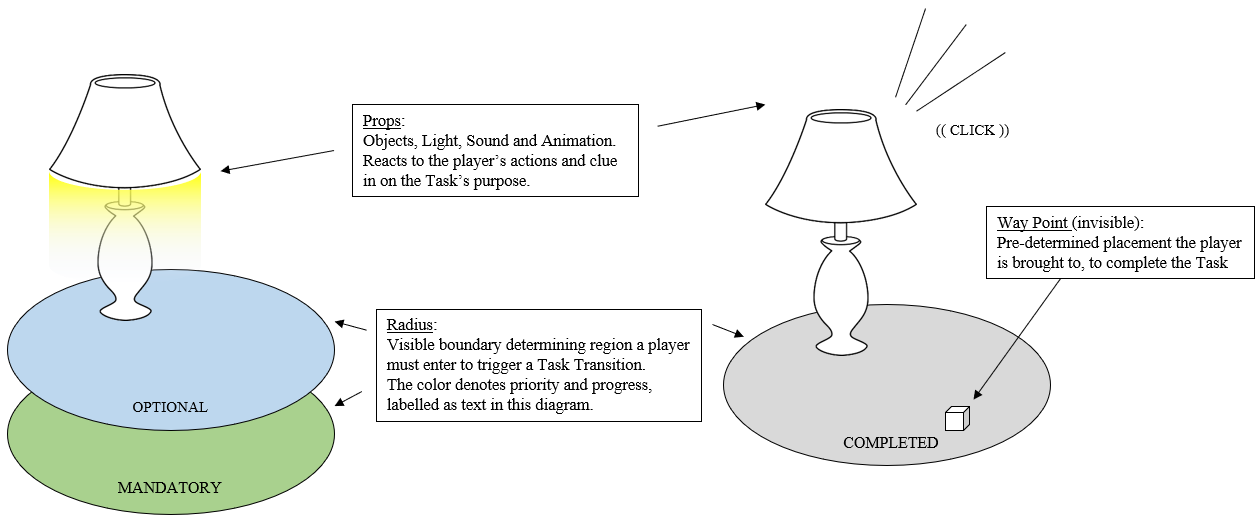
\includegraphics[width=0.95\paperwidth]{figures/InteractionSpaceDesign.png}
            \caption{\label{fig:FigureInteractionSpace}Overview of Interaction Space's Design Elements}               
    \end{figure}
    

\subsection{Player Character Design} \label{sec:develop_character}

    Given that the game was supposed to be a natural and immersive experience, no attention was desired to be brought to a character the user controls. Rather than creating one, the intent was to create an outward sense of belonging into the virtual world, as if the user could say “I am the character on-screen”. Implementing a person even just through aesthetic design could compromise that plan. This was the reason why the game was built with its first-person perspective, that would eliminate the need for any visible character traits on-screen or any latent thought of piloting something over those of self-control.\\
    However, merely showing nothing has one significant issue related to the novelty of the technology used. The Leap Motion is primarily used as an accessory apparatus to Virtual Reality experiences and games, and VR is itself a still uncommonly used technology, with many folks not having first hand experiences with it. The volunteers were predicted to not be completely aware of correct usage or limitations of the device unless if the game provided such feedback live as it occurs, and there isn’t enough time during a user trial to reach the level or proficiency required to innately recognize problems as they arise. A virtual representation of the player’s hand isn’t just a suggestion brought up by other applications of the Leap Motion device, but a requirement that must be present within the game, as then, the user is capable of discerning not just if they’re doing the correct gesture from the representation, but also if the application finds that they’re doing the correct gesture as well, or if small corrections will be required.\\
    Here, a decision is made that is at odds with the problem that caused the choice itself. What should the hand look like? There’re essentially only two possibilities: Either the hand looks realistically, but inevitably appears different from the user’s own real hand and a dissonance is established; or the hand is made to appear like an unambiguously digital approximation of a hand with simpler shapes. There were two at least two hand models provided by the Leap Motion’s library of assets that made either choice possible without much trouble. Given the two choices, no benefit is posed by the first option, and a lesser consistent experience among volunteers was predicted, not to mention the potential source for distraction provided by the more visually enticing.  There was a third option, giving the user a choice of hand model among a larger number, however, that could also pre-emptively give too much of an importance to the hand’s look, which is an undesirable outcome if avoidable. \\
    As such, during the game, the player can see a hand’s model built of simple gray and blue smooth shapes denoting fingers and joints, functioning as a proxy to the player’s own hand, and reacting to movement by performing the same gestures and staying at a similar depth and distance as the player’s own real hand would, mimicking a first person’s field of view with a raised hand.\\

    \begin{figure}[ht]
        \centering                                                
        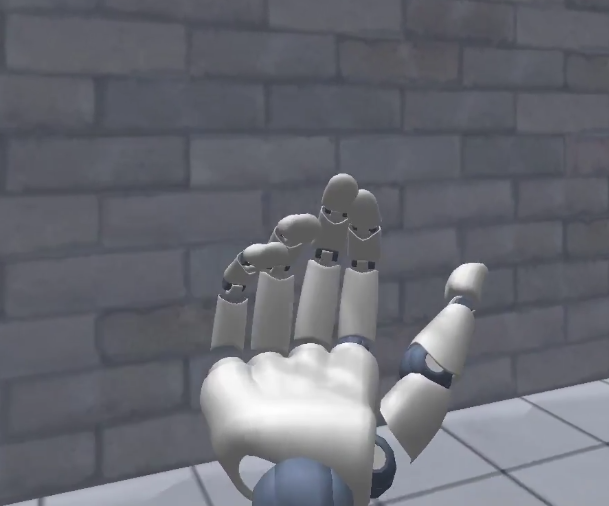
\includegraphics[width=0.3\paperwidth]{figures/HandIngame.png}
        \caption{\label{fig:FigureHand}Screen Capture of the in-game Hand Model}               
    \end{figure}

\subsection{Enviroment Design} \label{sec:develop_game_enviroment}

    The game occurs in a single virtual environment. Once it begins, there are no loading screens and any pauses happen only due to the game’s own interactive make up rather than to needing to load more assets. The only complex background processing required involves the classifier switching and even this should be a seamless and instant process. In other words, the game is small enough to be fully loaded at all times.
    Yet, it should also have been big enough that there isn’t a perception overload to the player with too many tasks and options present at a time. A large multiplicity of cues can confuse or frustrate the user. Given that there are 8 total tasks in the game separated in two groups of four, it was found appropriate to separate these into pairs of two tasks, one mandatory and one optional, and placed within four rooms. Additionally, to streamline the process of finding these tasks, the rooms were laid out in sequence through connecting corridors.\\
    
    \begin{figure}[ht]
        \centering
        \hspace*{-1cm}
        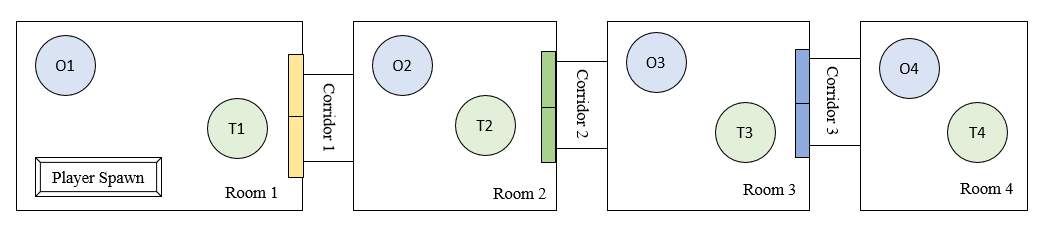
\includegraphics[width=0.8\paperwidth]{figures/RoomOverview.png}
        \caption{\label{fig:FigureRooms}Overview of the virtual enviroment's Room Design}
    \end{figure}

    One of the things that such a sequential line-up opens to the game is the chance of someone missing out on the presence of a task. This is undesirable, as detracting user choice from the completion of a task gives off less information about the task itself, than someone intentionally avoiding it or performing it and giving a bad grade. Opposed, to it, it does permit to observe one of the subtler factors of immersive experiences, assumingly, the user’s level of comfort and confidence with the controls, which are often overstated in self-assessments. Ultimately, the proposition of an intuitive cue for progress trumps over alternatives.\\
    Rooms are therefore separated by gates that do not open until the containing mandatory task is finished. Moreover, the transition between rooms is not just identified by the crossing of a gate, but also visually by the rooms themselves, as the looks of the floor, walls and ceilings changes drastically upon entering a corridor and matches with the following area. Also, to better attach the completion of a mandatory task with its correspondent gate, these gates were colored, and a key was integrated as part of the task’s completion.\\
    Other guiding elements are also present within rooms. Green arrows appear near gates, corridor entrances or on empty walls to help direct the user and reinforce that they’re heading the correct direction. Non-interactive plants are present on empty corner to fill the empty space and give the impression of a location of no interest to the game’s progress. Also, the empty play area with no object of interest is progressively funnelled in size, as the player is expected to make lesser mistakes in their movement as they progress and would find less of a reason to take large exploratory measures with the controls.\\ 
    This last point touches on the subject of room layout, which brings up the question of task placement. Of the two tasks in each room, the mandatory task is always placed closest to the exit gate and furthest to the entrance. The optional tasks however are progressively brought into the most direct path of the player. In order: O1 is on an indentation to the left of the room, O2 is off to the left but within the regular room boundaries, O3 is to the left of the path, but directly in front of the player from where they would come into the room, and finally, O4 is completely in the way of the player and they must sidestep it if they don’t want to compete the task. Additionally, O1 and O2 represent tasks that don’t lend themselves to having very much of an immediate urgency in nature, while O3 and O4 represent something that demands hurriedness from the user, and something that is just bothersome and has to be dealt with right away, thus justifying their progressive shift from staying away to getting in the way.\\
    
    \begin{figure}[ht]
        \centering
        \hspace*{-1cm}
        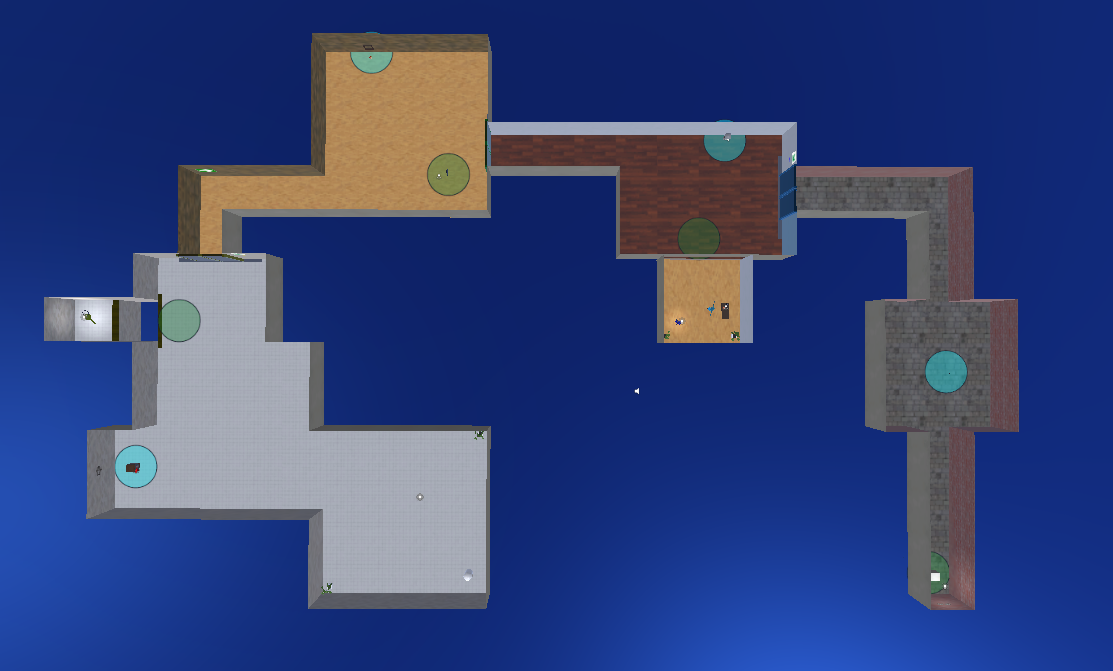
\includegraphics[width=0.8\paperwidth]{figures/Overhead.png}
        \caption{\label{fig:FigureGameOverhead}Overhead view of the game's virtual enviroment}
    \end{figure}

\subsection{Game Logic} \label{sec:develop_game_logic}
    For its implementation on Unity, the game has 4 core elements. These are the \emph{GameController}, \emph{CharacterController}, \emph{InteractionSpaceController} and \emph{CinematicHandler} scripts. Many other scripts were relevant to the game’s function, however, all of those had a small role within restrained contexts, and worked in a master, slave manner to one of these core scripts, such as, for example, the RadomFlight handler script, that made task O4’s insects move erratically, does not interact with any script besides the CinematicHandler and does so only on one moment in the game, during the closing transition of the O4 interaction space.\\
    The \emph{GameController} is tasked with initializing the game’s Shamanic Interface and defining state definitions that the game will require. It is also the game controller that will dispense a new classifier during task transitions. Thus, this Is an entry point for the Character Controller and the Interaction Space Controller during those times. It is also the GameController that defines the game’s culture, and it is here that I found the single difference between the game build presented to the Cultural and Non-Cultural groups. The Non-cultural group plays with an undefined Culture and thus the game uses the SI’s default gestures. Meanwhile, the Cultural group defines its culture as “PT” and those gestures get overridden by the pairs belonging to it. The code snippet corresponding to gesture efinition can be found on appendix \ref{ap1:InitCulturalLayer}. There’s a single Game Controller object in the game space and the other core scripts have a reference and access to it at any given moment.\\
    The Character Controller is a long script with definitions related to accepting input from the Leap Motion device (or Keyboard, for debugging purposes) to move the player’s camera around the virtual environment or to complete tasks. It’s here that the game checks if the classifier yields the correct gesture and if it’s also here that the game informs the rest of the system what gesture is currently being performed. It’s also where the game’s current valid options for control are changed, and where collision between a player and an interaction space’s region is handled. Ironically, the Character Controller is not statically aware of any command definition, merely matching what the classifier informs it, with the current Task. Its task completion code being agnostic to the definitions allows it to function if new definitions are set up. In summation, anything related to player input or to changing what a player can do has its entry point here.\\ 
    However, it’s the Interaction Space Controller that defines what those gestures are for each task, and if they’ve been performed for long enough to accrue to the task’s completion. While there is a single Character Controller there’s a different instance of the Interaction Space Controller attached to the corresponding game objects. Every interaction space object has its own script, with its own different internal settings correspondent to a different Task. Upon collision of the Player and an Interaction Script, the scripts belonging to each attach to each other, and a back process of communication ensues through the 3 Scripts. The Interaction Space controller informs the Character Controller of what Task is performed within the interaction space, and the Character Controller then requests the Game Controller To feed that task’s correspondent State into its Shamanic Interface. Finally, the Game Controller yields the resulting Classifier back to the Character Controller, and the Character Controller will from then on inform the Interaction Space every frame that a gesture was performed. State definition code snippets can be found in \ref{ap1:StateDefinitions}.\\
    This happens relatively instantaneously, albeit, there is some leeway to give the Shamanic Interface some time for returning the Classifier, as at the very first moment of the collision between player and Interaction Space, an initial task transition phase, called player repositioning, is executed. During these, the character controller actually removes control from the player for three seconds and forcefully moves them to an appropriate spot where they will perform the task’s gestures.\\
    And, finally, the Cinematic Handler, which synchs and performs visual and audible alterations to the environment during intermediate and final task transition phases. From moving and animating object, to dimming lights and turning off sounds, this provide the player with the feedback that a Task was completed by changing the task’s props in some manner. Only the Interaction Space Controller communicates with it, which means that granting player control after a Task’s completion must be done through it as a middleman between the Cinematic Handler and the Character Control Script.\\

    \begin{figure}[ht]
        \centering
        \hspace*{-1cm}
        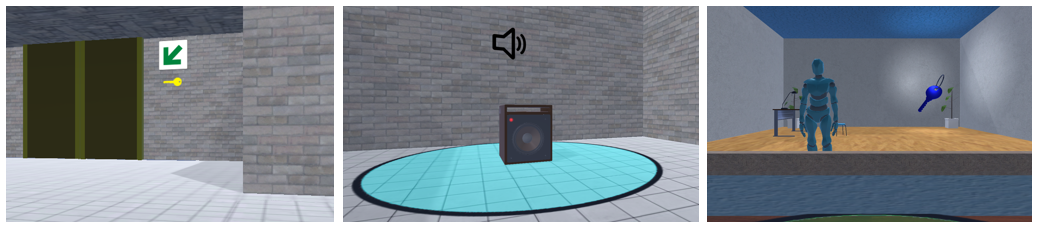
\includegraphics[width=0.8\paperwidth]{figures/IngameScreenshots.png}
        \caption{\label{fig:FigureScreenshots}Screenshots of the Game Enviroment}
    \end{figure}